\documentclass[conference]{IEEEtran}

% ---------- Packages ----------
\usepackage{amsmath, amssymb, graphicx, cite, hyperref}
\usepackage{tikz}
\usetikzlibrary{calc,arrows.meta,positioning,fit,shapes.geometric}
\usepackage{pgfplots}
\pgfplotsset{compat=1.18}
\usepackage{siunitx}

% ---------- Title ----------
\title{SkyEdge: Secure High-Altitude Drone Platform Integrating $H_\infty$ Control, Domestic Devices, and Advanced Mechanical Design}

% ---------- Author ----------
\author{
\IEEEauthorblockN{Shinichi Samizo}
\IEEEauthorblockA{Independent Semiconductor Researcher \\
Project Design Hub, Samizo-AITL \\
\textit{Email:} \href{mailto:shin3t72@gmail.com}{shin3t72@gmail.com} \\
\textit{GitHub:} \href{https://github.com/Samizo-AITL}{Samizo-AITL}}
}

\begin{document}
\maketitle

% ---------- Abstract ----------
\begin{abstract}
This paper presents the foundational design of \emph{SkyEdge}, 
a secure high-altitude unmanned aerial vehicle (UAV) platform that 
integrates $H_\infty$ control, domestic devices, and a variable-pitch 
mechanical structure. The proposed framework provides robust disturbance 
rejection, secure hardware implementation, and reliable flight capability 
up to 10{,}000 m altitude. We describe the control architecture, device 
integration, and mechanical design, and we outline evaluation plans 
toward a proof-of-concept prototype.
\end{abstract}

% ---------- Keywords ----------
\begin{IEEEkeywords}
UAV, robust control, $H_\infty$, variable-pitch rotor, secure systems, high-altitude flight
\end{IEEEkeywords}

% ---------- Sections ----------
\section{Introduction}
Unmanned aerial vehicles (UAVs) are increasingly important in defense, 
disaster response, and environmental monitoring. However, most commercial 
systems are limited to altitudes below 3{,}000 m, and many rely on 
foreign-made devices with security concerns. This paper aims to establish 
a domestic, secure UAV platform capable of robust operation in 
high-altitude environments.

\section{Related Work}
Control approaches such as PID, adaptive control, and sliding-mode 
control have been applied to UAVs, but robust performance under strong 
disturbances remains challenging. $H_\infty$ control has potential for 
disturbance rejection. Existing high-altitude UAV programs (NASA Helios, 
JAXA HAPS) demonstrate feasibility but rely on specialized designs. 
Security aspects and domestic device integration remain underexplored.

\section{System Architecture}
The proposed architecture integrates three layers:
\begin{itemize}
    \item \textbf{$H_\infty$ Control:} ensures robustness against gusts 
    up to 20--30 m/s.
    \item \textbf{FSM:} manages mode transitions (normal, high-altitude, 
    comm-loss, emergency return).
    \item \textbf{LLM:} assists adaptive redesign of control policies in 
    unforeseen conditions (simulation environment).
\end{itemize}

% ===================== Fig.1 (TWO columns) =====================
\begin{figure*}[t]
\centering
\resizebox{\textwidth}{!}{%
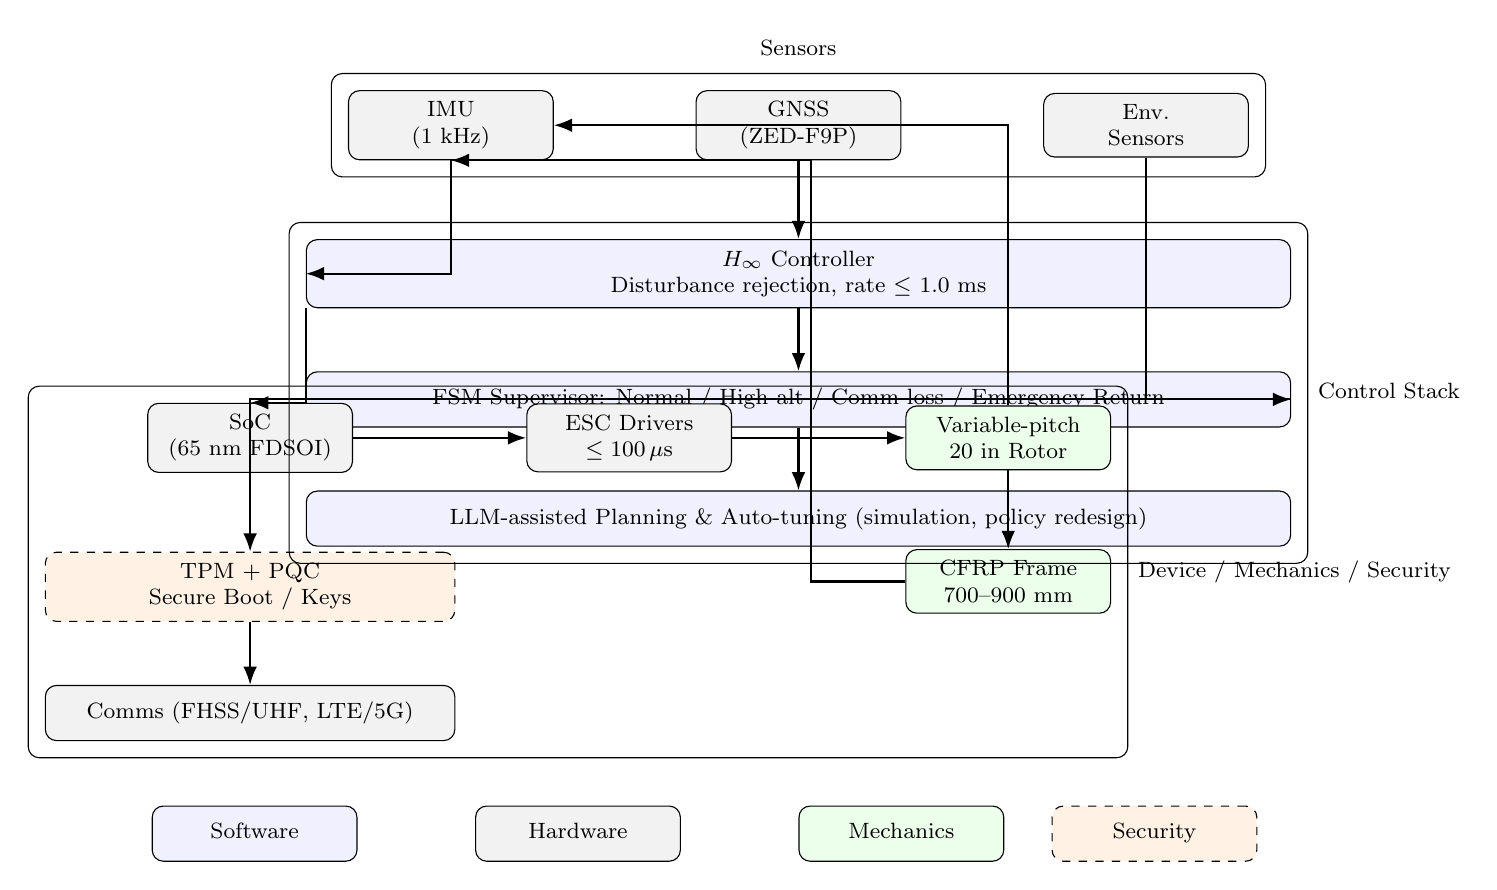
\begin{tikzpicture}[
    font=\footnotesize,
    node distance=8mm and 12mm,
    box/.style={draw, rounded corners, align=center, inner sep=4pt, minimum width=2.6cm, minimum height=7mm},
    hw/.style={box, fill=gray!10},
    sw/.style={box, fill=blue!6},
    mech/.style={box, fill=green!8},
    sec/.style={box, fill=orange!10, dashed},
    arrow/.style={-Latex, thick},
    grp/.style={draw, rounded corners, inner sep=6pt}
]

% ===== Sensors =====
\node[hw] (imu) {IMU\\(1 kHz)};
\node[hw, right=18mm of imu] (gps) {GNSS\\(ZED-F9P)};
\node[hw, right=18mm of gps] (env) {Env.\\Sensors};

% ===== H-infty control (inner loop) =====
\node[sw, below=10mm of gps, minimum width=12.5cm] (hinf) {$H_\infty$ Controller\\
Disturbance rejection, rate $\leq$ 1.0 ms};

% ===== FSM / LLM =====
\node[sw, below=8mm of hinf, minimum width=12.5cm] (fsm) {FSM Supervisor: Normal / High-alt / Comm-loss / Emergency Return};
\node[sw, below=8mm of fsm, minimum width=12.5cm] (llm) {LLM-assisted Planning \& Auto-tuning (simulation, policy redesign)};

% ===== Hardware stack (row) =====
\node[hw, below left=12mm and -6mm of hinf] (soc) {SoC\\(65 nm FDSOI)};
\node[hw, right=22mm of soc] (esc) {ESC Drivers\\$\leq 100\,\mu$s};
\node[mech, right=22mm of esc] (vp) {Variable-pitch\\20 in Rotor};

% ===== Mechanics / Security / Comms =====
\node[mech, below=10mm of vp] (frame) {CFRP Frame\\700--900 mm};
\node[sec, below=10mm of soc, minimum width=5.2cm] (secblk) {TPM + PQC\\Secure Boot / Keys};
\node[hw, below=8mm of secblk, minimum width=5.2cm] (comms) {Comms (FHSS/UHF, LTE/5G)};

% ===== Group boxes =====
\node[grp, fit=(imu)(gps)(env), label=above:{\strut Sensors}] (gSensors) {};
\node[grp, fit=(hinf)(fsm)(llm), label=right:{\strut Control Stack}] (gCtrl) {};
\node[grp, fit=(soc)(esc)(vp)(frame)(secblk)(comms),
      label=right:{\strut Device / Mechanics / Security}] (gHW) {};

% ===== Connections =====
\draw[arrow] (imu.south) |- (hinf.west);
\draw[arrow] (gps.south) -- (hinf.north);
\draw[arrow] (env.south) |- (fsm.east);

\draw[arrow] (hinf.south) -- (fsm.north);
\draw[arrow] (fsm.south) -- (llm.north);

\draw[arrow] (hinf.south west) |- (soc.north);
\draw[arrow] (soc.east) -- (esc.west);
\draw[arrow] (esc.east) -- (vp.west);
\draw[arrow] (vp.south) -- (frame.north);

\draw[arrow] (fsm.east) -| (secblk.north);
\draw[arrow] (secblk.south) -- (comms.north);

% Feedback
\draw[arrow] (frame.west) -| ++(-12mm,0) |- (imu.south);
\draw[arrow] (vp.north) |- (imu.east);

% ===== Legend (centered, no overlap) =====
\path (gHW.south) ++(0,-6mm) coordinate (leg);
\node[box, fill=blue!6,  anchor=north east] (lg1) at ($(leg)+(-28mm,0)$) {\strut Software};
\node[box, fill=gray!10, anchor=north]      (lg2) at (leg)               {\strut Hardware};
\node[box, fill=green!8, anchor=north west] (lg3) at ($(leg)+(28mm,0)$)   {\strut Mechanics};
\node[box, fill=orange!10, dashed, anchor=north west] (lg4)
      at ($(lg3.north east)+(6mm,0)$) {\strut Security};

\end{tikzpicture}%
}
\caption{SkyEdge system architecture (two-column figure). The three-layer control stack ($H_\infty$, FSM, LLM) integrates with sensors, a secure device stack (SoC, TPM/PQC, comms), and variable-pitch mechanical design.}
\label{fig:sysarch}
\end{figure*}

% ===================== Fig.2 (ONE column) =====================
\begin{figure}[t]
\centering
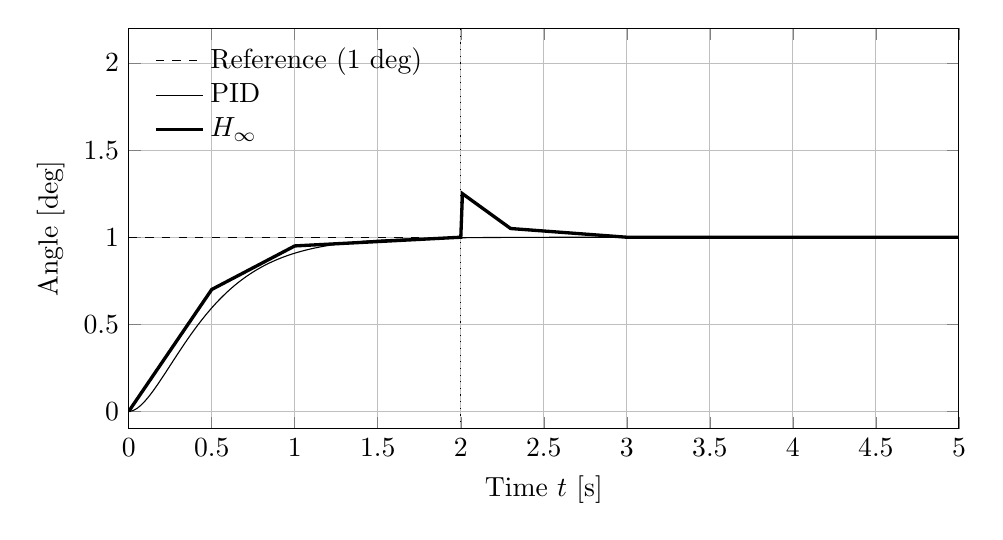
\begin{tikzpicture}
\begin{axis}[
    width=\columnwidth, height=0.55\columnwidth,
    xmin=0, xmax=5, ymin=-0.1, ymax=2.2,
    xlabel={Time $t$ [s]}, ylabel={Angle [deg]},
    grid=both,
    legend style={at={(0.02,0.98)},anchor=north west,draw=none,fill=none},
    legend cell align={left},
    ytick distance=0.5, xtick distance=0.5
]
% reference
\addplot[dashed] coordinates {(0,1) (5,1)};
\addlegendentry{Reference (1 deg)}

% PID(※ 角括弧あり!)
\addplot[smooth,domain=0:5,samples=200] {1 - exp(-4*x)*(1 + 4*x)};
\addlegendentry{PID}

% H-infinity response with gust at t=2 s
\addplot[very thick] coordinates
{(0,0) (0.5,0.7) (1,0.95) (2,1.0) (2.01,1.25) (2.3,1.05) (3,1.0) (5,1.0)};
\addlegendentry{$H_\infty$}

% gust marker
\draw[dotted] (axis cs:2,-0.1) -- (axis cs:2,2.2);
\end{axis}
\end{tikzpicture}
\caption{Step tracking with a sudden gust. The $H_\infty$ controller yields smaller overshoot and faster recovery than PID when a $+15\%$ gust hits at $t=2$ s.}
\label{fig:step}
\end{figure}

% ===================== Fig.3 (ONE column) =====================
\begin{figure}[t]
\centering
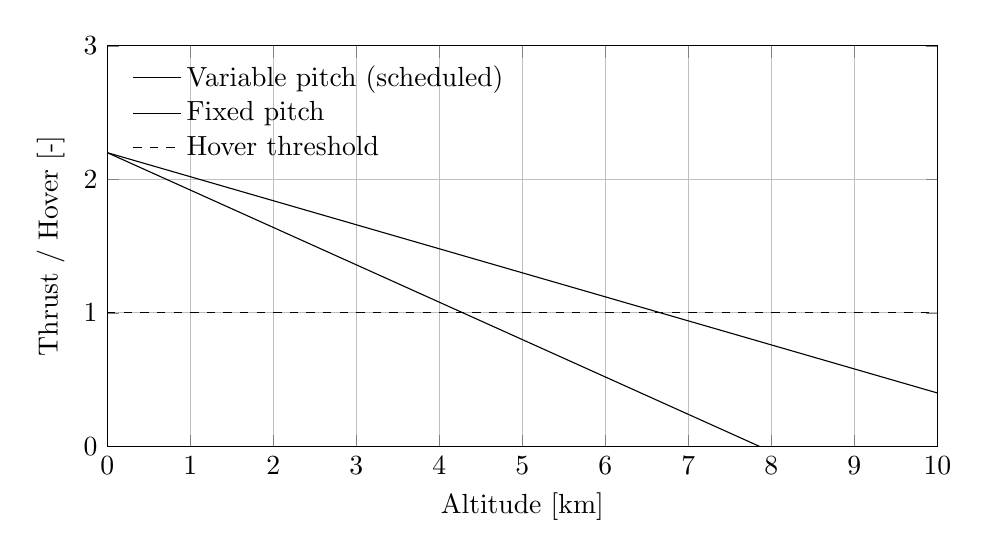
\begin{tikzpicture}
\begin{axis}[
    width=\columnwidth, height=0.55\columnwidth,
    xmin=0, xmax=10, ymin=0, ymax=3,
    xlabel={Altitude [km]}, ylabel={Thrust / Hover [-]},
    grid=both, legend style={at={(0.02,0.98)},anchor=north west,draw=none,fill=none},
    legend cell align={left}
]
\addplot[smooth,domain=0:10,samples=200] {2.2 - 0.18*x};      % variable pitch (scheduled)
\addlegendentry{Variable pitch (scheduled)}
\addplot[smooth,domain=0:10,samples=200] {2.2 - 0.28*x};      % fixed pitch
\addlegendentry{Fixed pitch}
\addplot[dashed] coordinates {(0,1) (10,1)};                   % hover threshold
\addlegendentry{Hover threshold}
\end{axis}
\end{tikzpicture}
\caption{Thrust margin vs. altitude. Pitch scheduling maintains margin above $1$ up to 10 km, while a fixed-pitch rotor loses margin.}
\label{fig:margin}
\end{figure}

% ===================== Fig.4 (ONE column) =====================
\begin{figure}[t]
\centering
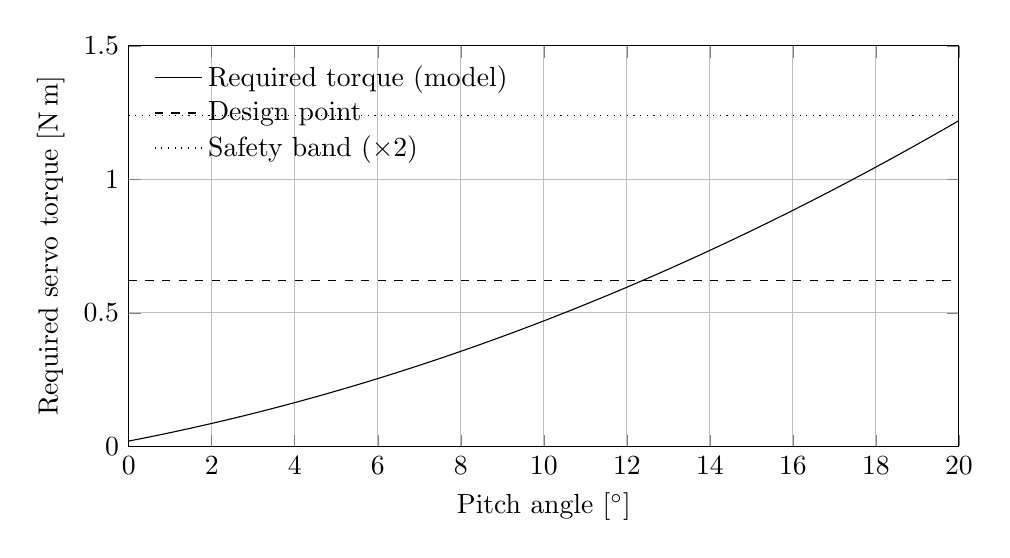
\begin{tikzpicture}
\begin{axis}[
    width=\columnwidth, height=0.55\columnwidth,
    xmin=0, xmax=20, ymin=0, ymax=1.5,
    xlabel={Pitch angle [\si{\degree}]}, ylabel={Required servo torque [N\,m]},
    grid=both, legend style={at={(0.02,0.98)},anchor=north west,draw=none,fill=none},
    legend cell align={left}
]
\addplot[smooth,domain=0:20,samples=200] {0.02 + 0.03*x + 0.0015*x*x};
\addlegendentry{Required torque (model)}
\addplot[dashed] coordinates {(0,0.62) (20,0.62)};
\addlegendentry{Design point}
\addplot[dotted] coordinates {(0,1.24) (20,1.24)};
\addlegendentry{Safety band ($\times 2$)}
\end{axis}
\end{tikzpicture}
\caption{Servo torque vs. pitch angle for the variable-pitch mechanism. The design point \SI{0.62}{N\,m} leaves a safety margin of $\times 2$.}
\label{fig:torque}
\end{figure}

% ===================== Fig.5 (ONE column) =====================
\begin{figure}[t]
\centering
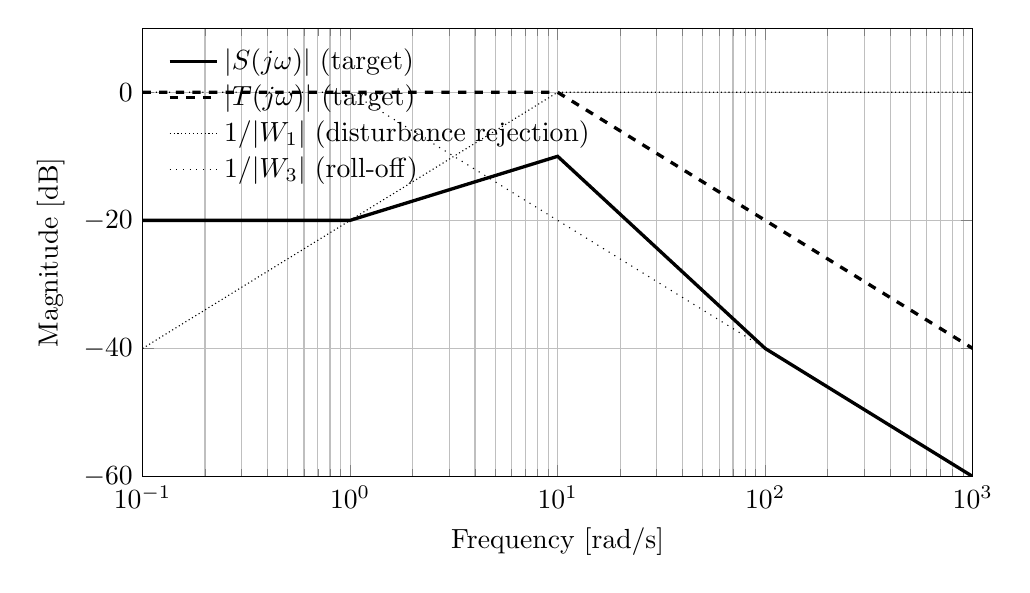
\begin{tikzpicture}
\begin{semilogxaxis}[
    width=\columnwidth, height=0.6\columnwidth,
    xmin=1e-1, xmax=1e3, ymin=-60, ymax=10,
    xlabel={Frequency [rad/s]}, ylabel={Magnitude [dB]},
    grid=both, legend style={at={(0.02,0.98)},anchor=north west,draw=none,fill=none},
    legend cell align={left}
]
% Target |S| and |T|
\addplot[very thick] coordinates {(0.1,-20) (1,-20) (10,-10) (100,-40) (1000,-60)};
\addlegendentry{$|S(j\omega)|$ (target)}
\addplot[dashed, very thick] coordinates {(0.1,0) (1,0) (10,0) (100,-20) (1000,-40)};
\addlegendentry{$|T(j\omega)|$ (target)}
% Weight hints
\addplot[densely dotted] coordinates {(0.1,-40) (1,-20) (10,0) (100,0) (1000,0)};
\addlegendentry{$1/|W_1|$ (disturbance rejection)}
\addplot[dotted] coordinates {(0.1,0) (1,0) (10,-20) (100,-40) (1000,-60)};
\addlegendentry{$1/|W_3|$ (roll-off)}
\end{semilogxaxis}
\end{tikzpicture}
\caption{Frequency-domain intuition for $H_\infty$ design: low $|S|$ at low--mid frequency (disturbance rejection) and low $|T|$ at high frequency (noise/roll-off).}
\label{fig:weights}
\end{figure}

% -------------------------------------------------------------
\section{Device Integration}
The device layer includes a domestic SoC (65 nm FDSOI), LDMOS motor 
drivers, high-rate IMU (1 kHz), and secure modules (TPM + PQC). 
Control cycle is maintained at $\leq 1.0$ ms with ESC response $\leq 100 
\, \mu$s. Estimated BOM cost is 596{,}700 JPY per unit (with reduction in 
mass production).

\section{Mechanical Design}
The UAV has a 700--900 mm frame, CFRP structure, and a variable-pitch 
20-inch rotor system. At take-off weight 6.38 kg, the thrust-to-weight 
ratio is $\approx 2.82$. Variable pitch enables adaptation from sea 
level to 10{,}000 m (RPM from $\approx 8{,}339$ to $14{,}353$). Servo torque 
requirement is 0.62 N$\cdot$m with safety factor of 2--3.

\section{Evaluation Plan}
Planned evaluations include wind-tunnel testing, low-temperature chamber 
tests, redundancy verification, and communication robustness under 
jamming scenarios. A proof-of-concept schedule has been drafted for 
2025--2026.

\section{Conclusion}
We presented the SkyEdge architecture integrating $H_\infty$ control, 
domestic devices, and mechanical design for secure high-altitude UAVs. 
The proposed system addresses robustness, security, and reliability at 
10{,}000 m operation. Future work includes prototype development and 
extension to underwater vehicles (\emph{SeaEdge}), toward a unified 
autonomous platform for defense, disaster response, GX, and education.

% ---------- References ----------
\bibliographystyle{IEEEtran}
\bibliography{refs}

\end{document}
